\documentclass[12pt]{article}

% Page layout
\usepackage{geometry}
\geometry{
  letterpaper,
  margin=1in
}

% Fonts and formatting
\usepackage{lmodern}
\usepackage{setspace}
\usepackage{xcolor}
\usepackage{tabularx}


% For better title control
\usepackage{titling}

\title{\vspace{2cm}
  \textbf{\Huge AstroStreet AR}\\[1em]
  \textbf{\Large Software Design Document (SDD)}\\[0.5em]
  \rule{0.8\textwidth}{0.5pt}\\[0.5em]
  \large CS 3338 -- Software Engineering Tools
}
\author{
  \large Group 2\\[0.5em]
  Royce Jamerson\\
  Khalid Jamil\\
  Michael Lieng\\
  Ricardo Ibanez
}
\date{\large December 11, 2025}

\usepackage{graphicx} % you may already have this
\usepackage{tikz}
\usetikzlibrary{arrows.meta, positioning}


\begin{document}

% ---------- Cover Page ----------
\begin{titlepage}
    \centering
    \vspace*{2cm}

    {\Huge \textbf{AstroStreet AR}\par}
    \vspace{0.8cm}
    {\Large \textbf{Software Design Document (SDD)}\par}
    \vspace{0.5cm}
    {\large Assignment 14\par}
    \vspace{0.5cm}
    {\large CS 3338 -- Software Engineering Tools\par}
    \vspace{0.5cm}
    {\large California State University, Los Angeles\par}

    \vfill

    {\large \textbf{Group 2}\par}
    \vspace{0.4cm}
    {\large Royce Jamerson\par}
    {\large Khalid Jamil\par}
    {\large Michael Lieng\par}
    {\large Ricardo Ibanez\par}

    \vfill

    {\large Date: December 11, 2025\par}

    \vspace*{1.5cm}
\end{titlepage}

% ---------- Table of Contents ----------
\pagenumbering{roman}        % Roman numerals for front matter
\setcounter{tocdepth}{2}     % Include sections and subsections
\tableofcontents
\newpage

\pagenumbering{arabic}       % Start normal page numbers for body

% ---------- SDD Sections (skeleton) ----------

% --- 1. Version Description
\section{Version Description}

This section tracks the revision history of the
\textit{AstroStreet AR} Software Design Document (SDD) for
Group 2 in CS 3338 -- Software Engineering Tools.

\begin{center}
\begin{tabularx}{\textwidth}{|c|X|c|}
\hline
\textbf{Version} & \textbf{Description} & \textbf{Date} \\
\hline
1.0 &
Initial version of the Software Design Document for
\textit{AstroStreet AR}, prepared for Assignment 14. &
December 2, 2025 \\
\hline
2.0 &
Expanded SDD with detailed component responsibilities, AR session lifecycle
and error handling, key runtime scenarios, and refined database design for
\textit{AstroStreet AR}. &
December 7, 2025 \\
\hline
3.0 &
Final version of the SDD including game state management details, UI
navigation flow, performance and resource considerations, and notes on
future extensibility (e.g., online leaderboards and additional game modes). &
December 11, 2025 \\
\hline
\end{tabularx}
\end{center}


Future revisions of this document can be recorded by adding new
rows to the table with updated version numbers, dates, and brief
descriptions of the changes.

% --- 2. Introduction
\section{Introduction}
\subsection{Purpose}

The purpose of this Software Design Document (SDD) is to describe the
overall design and internal structure of \textit{AstroStreet AR}, a
mobile augmented reality (AR) shooter game developed by Group 2 for
CS 3338 -- Software Engineering Tools at California State University,
Los Angeles.
This document translates the high-level requirements of the project into
a concrete design that can guide implementation, testing, and future
maintenance.

\subsection{System Overview}

\textit{AstroStreet AR} is a smartphone game in which players go
outside, use their phone's camera, and see virtual asteroids and alien
ships overlaid on the real world.
The player rotates their body and phone to aim and taps on the screen to
fire projectiles and destroy incoming targets.
The game tracks score, player health or shields, and increasing
difficulty as more enemies appear over time.

At a high level, the system consists of:
\begin{itemize}
    \item A mobile client that renders the AR scene, handles user input,
    manages game logic, and displays the user interface.
    \item AR services provided by the underlying platform
    (e.g., ARCore/ARKit via an engine such as Unity) to track device
    position and orientation and to overlay virtual objects on the
    camera feed.
    \item Local data storage to persist high scores and basic player
    settings on the device.
\end{itemize}

\subsection{Intended Audience}

This document is intended for:
\begin{itemize}
    \item Members of Group 2, who will use the design as a blueprint for
    implementing \textit{AstroStreet AR}.
    \item The course instructor and teaching staff, who will review the
    design as part of Assignment 14.
    \item Future developers or maintainers who may extend the game's
    features, port it to new platforms, or integrate additional
    services (such as online leaderboards).
\end{itemize}

\subsection{Document Overview}

The remainder of this SDD is organized as follows:
\begin{itemize}
    \item \textbf{System Architecture} describes the major components of
    \textit{AstroStreet AR}, their responsibilities, and how they
    interact.
    \item \textbf{User Interface} presents the planned screens and HUD
    elements, including the main menu, AR gameplay view, and score
    displays.
    \item \textbf{Database Design and Explanation} outlines the data
    structures used to store high scores and game settings, and explains
    how the application accesses this data.
    \item \textbf{Glossary} defines key technical terms and acronyms
    used throughout the document.
    \item \textbf{References} lists external resources, documentation,
    and tools consulted while designing \textit{AstroStreet AR}.
\end{itemize}

% --- 3. System Architecture
\section{System Architecture}
\subsection{Architecture Overview}

The architecture of \textit{AstroStreet AR} is organized around a
single mobile client application that runs on a smartphone and
communicates with platform-specific AR services.
Within the client, the game is decomposed into modular components
that manage AR tracking, game state, enemy behavior, player input,
user interface, and local data storage.

At a high level, the system consists of the following layers:
\begin{itemize}
    \item \textbf{Presentation Layer}: Responsible for rendering the
    camera feed, drawing virtual objects (asteroids, alien ships,
    projectiles), and displaying the heads-up display (HUD) and menus.
    \item \textbf{Game Logic Layer}: Manages the core game loop,
    including spawning enemies, updating the player state, handling
    collisions, tracking score, and determining win/lose conditions.
    \item \textbf{AR and Device Services Layer}: Interfaces with the
    underlying AR framework (e.g., ARCore/ARKit via Unity) to obtain
    camera images, device pose (position and orientation), and other
    sensor data.
    \item \textbf{Data Layer}: Handles reading and writing persistent
    data, such as high scores and basic settings, on the device.
\end{itemize}

Figure~\ref{fig:architecture} conceptually illustrates the relationships
between the major components.

\begin{figure}[h]
    \centering
    \resizebox{0.9\textwidth}{!}{%
    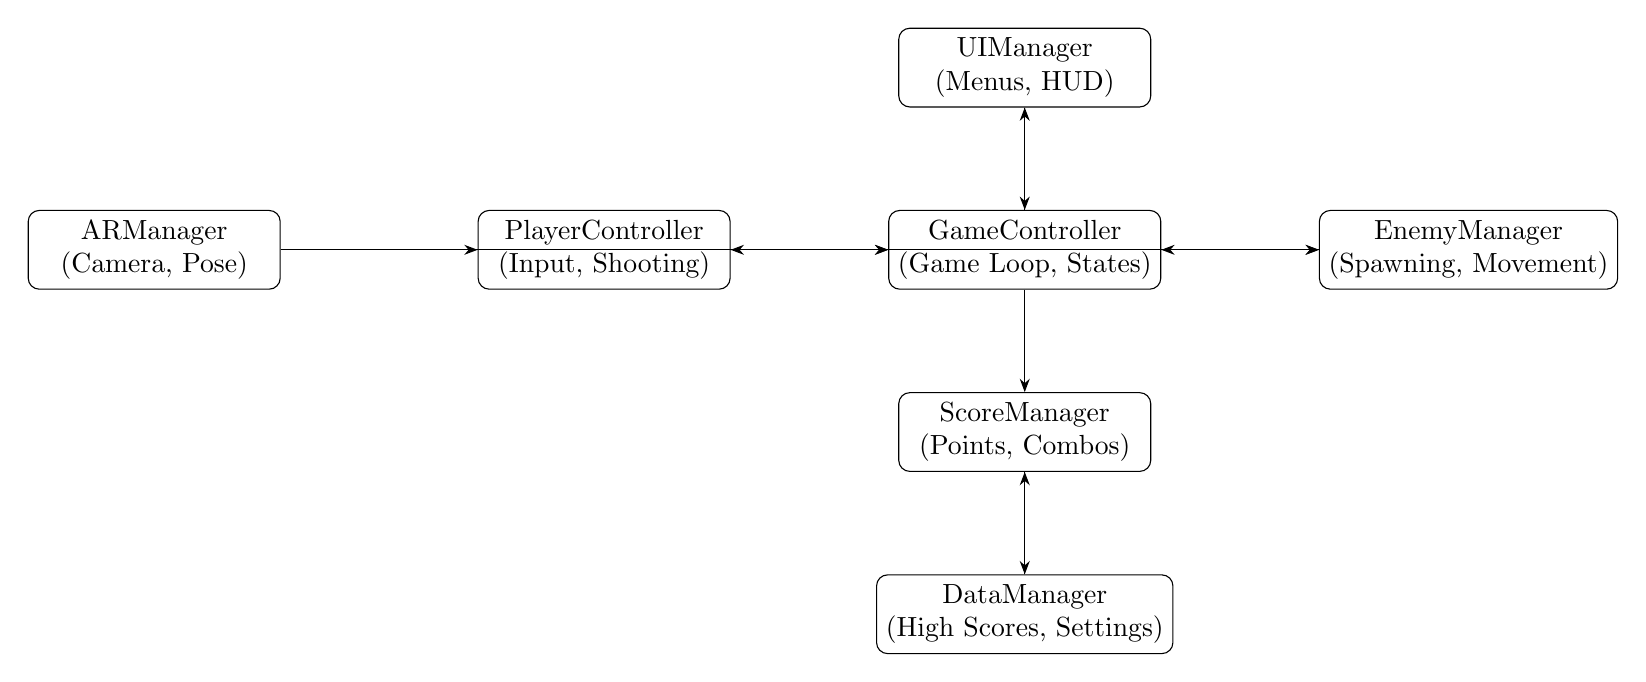
\begin{tikzpicture}[
        component/.style={
            rectangle,
            draw,
            rounded corners,
            minimum width=3.2cm,
            minimum height=1cm,
            align=center
        },
        >=Stealth,
        node distance=1.3cm and 2.0cm
    ]

    % Nodes
    \node[component] (ui) {UIManager\\(Menus, HUD)};
    \node[component, below=of ui] (game) {GameController\\(Game Loop, States)};
    \node[component, left=of game] (player) {PlayerController\\(Input, Shooting)};
    \node[component, right=of game] (enemy) {EnemyManager\\(Spawning, Movement)};
    \node[component, below=of game] (score) {ScoreManager\\(Points, Combos)};
    \node[component, below=of score] (data) {DataManager\\(High Scores, Settings)};
    \node[component, left=of player, xshift=-0.5cm] (ar) {ARManager\\(Camera, Pose)};

    % Arrows to/from GameController
    \draw[->] (ui) -- (game);
    \draw[->] (game) -- (ui);

    \draw[->] (player) -- (game);
    \draw[->] (game) -- (player);

    \draw[->] (enemy) -- (game);
    \draw[->] (game) -- (enemy);

    \draw[->] (game) -- (score);

    \draw[->] (score) -- (data);
    \draw[->] (data) -- (score);

    \draw[->] (ar) -- (game);
    \draw[->] (ar) -- (enemy);
    \draw[->] (ar) -- (player);

    \end{tikzpicture}
    }% end resizebox
    \caption{High-level component architecture of \textit{AstroStreet AR}.}
    \label{fig:architecture}
\end{figure}



\subsection{Major Components}

The main components of the client application are described below.

\subsubsection{ARManager}

The \textbf{ARManager} is responsible for:
\begin{itemize}
    \item Initializing the AR session when the game starts.
    \item Accessing the device camera feed and sensor data from the AR
    framework.
    \item Providing the current device pose (position and orientation)
    so that virtual objects can be placed consistently in the player's
    view.
\end{itemize}
Other components (such as the \textbf{GameController} and
\textbf{EnemyManager}) rely on the \textbf{ARManager} to ensure that
objects are rendered relative to the player's real-world orientation.

\subsubsection{GameController}

The \textbf{GameController} coordinates the overall game loop:
\begin{itemize}
    \item Starting and stopping gameplay sessions.
    \item Updating the game state each frame (time remaining, player
    health or shields, active enemies, and projectiles).
    \item Notifying other components when the game transitions between
    states (e.g., from ``Main Menu'' to ``In Game'' to ``Game Over'').
\end{itemize}
It serves as the central point of control, invoking the
\textbf{EnemyManager}, \textbf{PlayerController}, and
\textbf{UIManager} as needed during each update cycle.

\subsubsection{EnemyManager}

The \textbf{EnemyManager} handles all enemy-related behavior:
\begin{itemize}
    \item Spawning asteroids and alien ships according to the current
    difficulty level.
    \item Updating enemy movement and checking when enemies become too
    close to the player.
    \item Informing the \textbf{GameController} when enemies are
    destroyed or when they collide with the player.
\end{itemize}
The \textbf{EnemyManager} uses AR pose information from the
\textbf{ARManager} to decide where to place enemies in the player's
field of view.

\subsubsection{PlayerController}

The \textbf{PlayerController} interprets user input and updates the
player's actions:
\begin{itemize}
    \item Reading touch input (e.g., tapping the screen to shoot).
    \item Aligning the virtual crosshair or reticle with the player's
    current viewing direction.
    \item Requesting the creation of projectiles when the player fires
    and reporting hits back to the \textbf{GameController}.
\end{itemize}
It acts as the bridge between physical device movements/touches and
in-game actions.

\subsubsection{UIManager}

The \textbf{UIManager} manages the user interface and HUD:
\begin{itemize}
    \item Displaying the main menu, pause menu, and game over screen.
    \item Rendering HUD elements during gameplay, such as the score,
    health or shield bar, time remaining, and any active power-ups.
    \item Receiving navigation commands from the user (e.g., starting a
    new game, returning to the main menu).
\end{itemize}
The \textbf{UIManager} communicates with the \textbf{GameController}
and \textbf{ScoreManager} to update visual information.

\subsubsection{ScoreManager}

The \textbf{ScoreManager} tracks and updates the player's score:
\begin{itemize}
    \item Awarding points when enemies are destroyed.
    \item Applying score multipliers or bonuses for streaks.
    \item Exposing the current score to the \textbf{UIManager} for
    display during gameplay.
\end{itemize}
At the end of a game session, the \textbf{ScoreManager} collaborates
with the \textbf{DataManager} to save high scores.

\subsubsection{DataManager}

The \textbf{DataManager} is responsible for:
\begin{itemize}
    \item Persisting high scores and basic settings (such as sound
    preferences and control sensitivity) to local storage on the
    device.
    \item Loading saved data when the application starts.
    \item Providing a simple interface for other components to read and
    write data without dealing directly with the storage mechanism.
\end{itemize}

\subsection{Component Interactions}

During a typical gameplay session, the components interact as follows:
\begin{enumerate}
    \item The user selects ``Start Game'' from the main menu.
          The \textbf{UIManager} notifies the \textbf{GameController}
          to begin a new session.
    \item The \textbf{GameController} initializes the game state and
          requests the \textbf{ARManager} to start the AR session.
    \item The \textbf{EnemyManager} begins spawning enemies in positions
          derived from the AR pose provided by the \textbf{ARManager}.
    \item Each frame, the \textbf{PlayerController} reads user input
          (screen taps) and creates projectiles along the player's
          current viewing direction.
    \item The \textbf{GameController} updates all active entities,
          checks for collisions between projectiles and enemies, and
          adjusts the player's health or shields if enemies get too
          close.
    \item The \textbf{ScoreManager} updates the score when enemies are
          destroyed, and the \textbf{UIManager} refreshes the HUD to
          show the latest score and health values.
    \item When the game ends (e.g., the player's health reaches zero),
          the \textbf{GameController} notifies the \textbf{ScoreManager}
          and \textbf{DataManager} to save the final score, then
          instructs the \textbf{UIManager} to display the game over
          screen.
\end{enumerate}

This modular architecture is intended to keep responsibilities clearly
separated, making the system easier to implement, test, and extend with
future features such as additional enemy types, power-ups, or online
leaderboards.

\subsection{Component Responsibilities}

The AstroStreet AR system is organized into a small set of core components.
Each component has a clear set of responsibilities and limited knowledge of
other components in order to keep the design modular and maintainable.

Table~\ref{tab:component-responsibilities} summarizes the main runtime
components and how they collaborate.

\begin{table}[H]
  \centering
  \caption{Core Component Responsibilities}
  \label{tab:component-responsibilities}
  \begin{tabular}{|l|p{6cm}|p{4cm}|}
    \hline
    \textbf{Component} & \textbf{Responsibilities} & \textbf{Collaborates With} \\
    \hline
    \texttt{GameManager} &
    Owns the overall game state (e.g., Main Menu, Playing, Paused, Game Over).
    Initializes subsystems on game start, triggers wave progression, and
    coordinates transitions between screens. &
    \texttt{EnemyManager}, \texttt{PlayerController}, \texttt{UIManager},
    \texttt{DataManager}, \texttt{ARController} \\
    \hline
    \texttt{EnemyManager} &
    Spawns, updates, and removes enemies (asteroids and alien ships) within the
    AR scene. Controls enemy wave logic, difficulty scaling, and despawn rules
    when enemies move out of range or time out. &
    \texttt{GameManager}, \texttt{ARController} \\
    \hline
    \texttt{PlayerController} &
    Reads device input (screen taps) and device pose/orientation from the AR
    subsystem. Responsible for firing projectiles in the current view
    direction and notifying the \texttt{GameManager} when a hit occurs. &
    \texttt{GameManager}, \texttt{ARController}, \texttt{UIManager} \\
    \hline
    \texttt{UIManager} &
    Manages all UI screens (Main Menu, AR HUD, Pause Menu, Game Over, Settings,
    High Scores). Updates on-screen information such as score, health, and wave
    number based on notifications from the \texttt{GameManager}. &
    \texttt{GameManager}, \texttt{DataManager} \\
    \hline
    \texttt{DataManager} &
    Provides a simple persistence API for saving and loading local data such as
    high scores, basic player statistics, and user settings. Hides the
    underlying storage mechanism (e.g., SQLite or key--value store) from the
    rest of the system. &
    \texttt{GameManager}, \texttt{UIManager} \\
    \hline
    \texttt{ARController} &
    Wraps the underlying AR SDK (e.g., ARCore/ARKit via Unity AR Foundation).
    Manages the AR session lifecycle, pose tracking, and raycasts. Provides
    utility methods to place enemies and projectiles in world space relative to
    the player's real-world position and orientation. &
    \texttt{GameManager}, \texttt{EnemyManager}, \texttt{PlayerController} \\
    \hline
  \end{tabular}
\end{table}

By clearly separating responsibilities into these components, the team can
modify game rules, UI behavior, or persistence details with minimal impact on
the AR integration layer, and vice versa.

\subsection{AR Session Lifecycle and Error Handling}

AstroStreet AR relies on a mobile AR session to align virtual enemies and
projectiles with the player's physical environment. The \texttt{ARController}
encapsulates the AR session lifecycle and exposes a simplified interface to the
rest of the game.

At a high level, the AR session progresses through the following states:

\begin{itemize}
  \item \textbf{Not Initialized}: The app has launched, but no AR session has
  been created yet. The \texttt{GameManager} displays the Main Menu during this
  state.

  \item \textbf{Initializing}: After the player taps ``Start Game'', the
  \texttt{ARController} requests camera permissions (if needed), configures the
  AR session, and begins tracking.

  \item \textbf{Tracking}: The AR SDK reports a stable pose and tracking state.
  Enemies can be spawned at positions derived from detected planes or from the
  device's forward direction, and gameplay proceeds normally.

  \item \textbf{Limited / Lost Tracking}: The AR SDK reports that tracking is
  degraded (e.g., due to low light, fast motion, or lack of visual features).
  During this state, the game temporarily pauses spawning new enemies and may
  reduce or pause collision checks to avoid jarring behavior.
\end{itemize}

The \texttt{ARController} periodically reports the current tracking status to
the \texttt{GameManager}. When tracking is limited or lost, the
\texttt{UIManager} displays a simple overlay message such as
``Move your phone slowly'' or ``Point your camera at a textured surface''. Once
tracking returns to the \textbf{Tracking} state, normal gameplay resumes.

If the player denies camera or AR permissions, or if the device cannot support
AR, the \texttt{ARController} reports a fatal initialization error to the
\texttt{GameManager}. In this case, the \texttt{UIManager} shows an error
dialog and routes the user back to the Main Menu, where they can either retry
or exit the game.

\subsection{Key Runtime Scenarios}

This subsection describes two core runtime scenarios in terms of the
collaboration between components. These scenarios serve as an informal
sequence-diagram-style description.

\subsubsection{Starting a New AR Game Session}

\begin{enumerate}
  \item The player launches the app and sees the Main Menu rendered by the
  \texttt{UIManager}.
  \item The player taps the ``Start Game'' button.
  \item The \texttt{UIManager} notifies the \texttt{GameManager} that a new
  game has been requested.
  \item The \texttt{GameManager} instructs the \texttt{ARController} to start
  the AR session. The \texttt{ARController} requests permissions if necessary
  and transitions through the \textbf{Initializing} state into
  \textbf{Tracking}.
  \item Once tracking is stable, the \texttt{GameManager} updates its internal
  state to \textbf{Playing} and tells the \texttt{UIManager} to display the AR
  HUD.
  \item The \texttt{EnemyManager} begins spawning enemies at positions computed
  via the \texttt{ARController} (e.g., in front of the player's current pose or
  on detected planes).
\end{enumerate}

\subsubsection{Firing at an Enemy and Updating the Score}

\begin{enumerate}
  \item While in the \textbf{Playing} state, the player taps on the screen.
  \item The \texttt{PlayerController} receives the tap input and queries the
  \texttt{ARController} for the current device pose and forward direction.
  \item The \texttt{PlayerController} spawns a projectile traveling along the
  forward direction and registers it with the game world.
  \item During the next update cycle, the game checks for collisions between
  projectiles and enemies managed by the \texttt{EnemyManager}.
  \item If a collision is detected, the \texttt{EnemyManager} removes the enemy
  and notifies the \texttt{GameManager} that an enemy has been destroyed.
  \item The \texttt{GameManager} increments the player's score and updates any
  wave-related counters. It then instructs the \texttt{UIManager} to refresh
  the on-screen score display.
  \item At the end of the session (e.g., when the player runs out of health),
  the \texttt{GameManager} compares the final score against previously saved
  high scores via the \texttt{DataManager}. If a new high score is achieved,
  the \texttt{DataManager} persists it before the \texttt{UIManager} transitions
  to the Game Over screen.
\end{enumerate}

\subsection{Game State Management}

AstroStreet AR uses an explicit game state model to keep the behavior of the
\texttt{GameManager} predictable and easy to modify. The main high-level states
are:

\begin{itemize}
  \item \textbf{MainMenu}: The player is on the title screen and can choose to
  start a game, view high scores, open settings, or quit.
  \item \textbf{InitializingAR}: The game has received a request to start a new
  game and is waiting for the AR session to initialize and reach a stable
  tracking state.
  \item \textbf{Playing}: The AR session is active, enemies are spawning, and
  the player can move, aim, and fire.
  \item \textbf{Paused}: Gameplay is temporarily suspended; enemies and
  projectiles stop updating and the Pause Menu is visible.
  \item \textbf{GameOver}: The player has lost all health or another end
  condition has been reached; the final score is shown and may be saved.
\end{itemize}

State transitions are driven by player actions and AR session events. At a high
level:

\begin{itemize}
  \item \textbf{MainMenu $\rightarrow$ InitializingAR}: Player taps ``Start
  Game''.
  \item \textbf{InitializingAR $\rightarrow$ Playing}: The \texttt{ARController}
  reports that tracking has reached a stable state.
  \item \textbf{Playing $\rightarrow$ Paused}: Player taps the pause button or
  the app is backgrounded.
  \item \textbf{Paused $\rightarrow$ Playing}: Player selects ``Resume'' from
  the Pause Menu.
  \item \textbf{Playing $\rightarrow$ GameOver}: Player health reaches zero or
  another game-ending condition is met.
  \item \textbf{GameOver $\rightarrow$ MainMenu}: Player confirms going back to
  the main menu after reviewing their score.
\end{itemize}

The \texttt{GameManager} owns the current game state and exposes methods such
as \texttt{StartNewGame()}, \texttt{PauseGame()}, and \texttt{EndGame()}.
Other components (e.g., \texttt{UIManager}, \texttt{EnemyManager}) react to
state changes via simple notifications, which keeps state transitions
centralized and reduces the risk of inconsistent behavior.

\subsection{Performance and Resource Considerations}

As a mobile AR title, AstroStreet AR must balance visual fidelity with
performance and battery usage. The following design decisions aim to keep the
experience smooth on typical student devices:

\begin{itemize}
  \item \textbf{Target Frame Rate}: The game targets at least 30 frames per
  second during gameplay. Enemy spawn rates, projectile counts, and particle
  effects are tuned so that the total number of active objects remains within a
  safe limit.
  \item \textbf{Object Pooling}: Frequently created and destroyed objects such
  as projectiles are good candidates for object pooling. Instead of allocating
  and freeing these objects every time, the system can reuse a small pool to
  reduce garbage collection overhead.
  \item \textbf{Capped Enemy Count}: The \texttt{EnemyManager} enforces a
  maximum number of active enemies at any given time. When the cap is reached,
  new enemies are not spawned until existing enemies are destroyed or
  despawned.
  \item \textbf{Lightweight UI}: HUD elements use simple text and shapes rather
  than heavy animations to minimize overdraw. This is particularly important
  because the camera feed itself already fills the background.
  \item \textbf{AR Query Throttling}: Expensive AR queries (such as plane
  detection or raycasting) are performed at a limited frequency instead of
  every frame, providing a balance between responsiveness and performance.
\end{itemize}

These considerations are not exhaustive, but they define a baseline performance
profile that can be refined in future iterations without requiring a major
rewrite of the core architecture.

\subsection{Extensibility and Future Enhancements}

Although the current implementation of AstroStreet AR focuses on a single--player,
local high-score experience, the design intentionally leaves room for future
extensions. Examples include:

\begin{itemize}
  \item \textbf{Online Leaderboards}: The existing \texttt{HighScore} and
  \texttt{PlayerStats} entities can be synchronized with a remote service.
  The \texttt{DataManager} would act as a façade in front of both local and
  remote storage without requiring major changes to the rest of the game.
  \item \textbf{Additional Enemy Types and Behaviors}: New enemies with
  different movement patterns or attack styles can be added by extending the
  \texttt{EnemyManager} and related enemy components. The overall architecture
  (AR placement, game state management) remains unchanged.
  \item \textbf{New Game Modes}: Timed challenges, endless modes, or
  wave-based progression systems can be introduced primarily by updating the
  \texttt{GameManager}'s state transitions and scoring logic.
  \item \textbf{Accessibility Options}: Additional settings such as colorblind
  modes, adjustable HUD sizes, or alternative input schemes can be added by
  extending the \texttt{Settings} entity and updating the \texttt{UIManager}.
\end{itemize}

By documenting these potential extensions, the final SDD provides guidance for
future contributors who may wish to grow AstroStreet AR beyond the scope of the
course project.


% --- 4. User Interface 
\section{User Interface}

\subsection{Overview}

The user interface (UI) of \textit{AstroStreet AR} is designed to be
simple and usable outdoors while the player is holding a smartphone.
Navigation is primarily tap-based, and the most important information
(score, health, and basic controls) is always visible during gameplay.

The main UI elements include:
\begin{itemize}
    \item A \textbf{main menu} for starting the game and accessing other
    screens.
    \item An \textbf{AR gameplay view} that overlays enemies and HUD
    elements on top of the camera feed.
    \item A \textbf{pause menu} for temporarily stopping gameplay.
    \item A \textbf{game over screen} that summarizes the player's
    performance.
    \item A \textbf{high scores} screen.
    \item A \textbf{settings} screen for basic configuration options.
\end{itemize}

\subsection{Main Menu}

When the application launches, the user is shown the main menu screen.
This screen contains:
\begin{itemize}
    \item The game title: \textbf{AstroStreet AR}.
    \item A brief subtitle or tagline (e.g., ``Aim at the sky and blast
    incoming asteroids!'').
    \item A set of buttons:
    \begin{itemize}
        \item \textbf{Start Game} -- begins a new AR gameplay session.
        \item \textbf{High Scores} -- opens the high scores screen.
        \item \textbf{Settings} -- opens the settings screen.
        \item \textbf{Exit} (optional on platforms that support it) --
        closes the application.
    \end{itemize}
\end{itemize}

The main menu is displayed on top of a static or subtly animated
background image related to outer space or the night sky.
From this screen, the player can reach all other major UI flows.

\subsection{AR Gameplay Screen}

The AR gameplay screen is the core of the user experience.
It uses the device camera feed as the background and overlays virtual
game elements on top.

The key elements of this screen are:
\begin{itemize}
    \item \textbf{Camera View}: The live camera feed fills the entire
    screen to show the player's real-world surroundings.
    \item \textbf{Crosshair or Reticle}: A small graphical reticle is
    centered on the screen and indicates where the player's shots are
    aimed.
    \item \textbf{Score Display}: The current score is shown in the
    upper-left corner of the screen.
    \item \textbf{Health or Shield Bar}: The player's remaining health
    or shield is represented as a bar or set of segments in the
    upper-right corner.
    \item \textbf{Timer} (if used): If the game mode uses a time limit,
    the remaining time is displayed near the top of the screen.
    \item \textbf{Pause Button}: A small pause icon appears in one
    corner (e.g., top-right), allowing the user to open the pause menu.
\end{itemize}

To interact with this screen, the user:
\begin{itemize}
    \item Physically rotates or tilts the phone to aim the reticle at
    enemies that are rendered in the AR view.
    \item Taps the screen to fire projectiles in the direction of the
    reticle.
\end{itemize}

Enemies (asteroids and alien ships), projectiles, explosions, and
power-ups are all rendered as virtual objects anchored in the AR scene.

\subsection{Pause Menu}

The pause menu appears when the user taps the pause button during
gameplay.
When the game is paused, the AR scene is dimmed or frozen, and a small
overlay panel is shown with the following options:
\begin{itemize}
    \item \textbf{Resume} -- returns to the AR gameplay screen and
    continues the session.
    \item \textbf{Settings} -- opens a subset of settings (for example,
    sound on/off and sensitivity) without leaving the session.
    \item \textbf{Quit to Main Menu} -- ends the current game and
    returns to the main menu.
\end{itemize}

\subsection{Game Over Screen}

When the player's health reaches zero or the game session ends for
another reason (such as a time limit), the game over screen is shown.

This screen contains:
\begin{itemize}
    \item A prominent ``Game Over'' title.
    \item The player's final score.
    \item An indication if a new high score was achieved.
    \item Buttons for:
    \begin{itemize}
        \item \textbf{Play Again} -- start a new game session.
        \item \textbf{Return to Main Menu} -- go back to the main menu.
    \end{itemize}
\end{itemize}

\subsection{High Scores Screen}

The high scores screen displays a list of the top scores recorded on
the device.
A simple layout might include:
\begin{itemize}
    \item A title such as ``High Scores''.
    \item A table or vertical list showing rank, score value, and date
    achieved.
    \item A button to return to the main menu.
\end{itemize}

\subsection{Settings Screen}

The settings screen allows the user to adjust basic configuration
options for \textit{AstroStreet AR}.
Possible settings include:
\begin{itemize}
    \item \textbf{Sound}: toggle sound effects on or off.
    \item \textbf{Control Sensitivity}: adjust how quickly the reticle
    responds to device movement.
    \item \textbf{Brightness or UI Contrast}: optional adjustments to
    help make the HUD more readable outdoors.
\end{itemize}

The settings screen is accessible from both the main menu and the pause
menu, and includes a button to return to the previous screen.

Overall, the user interface is designed to minimize on-screen clutter so
that players can clearly see both the real world and the virtual
objects they are interacting with while playing \textit{AstroStreet AR}.

\subsection{UI Navigation Flow}

The user interface is organized around a small set of screens connected in a
simple, predictable flow. This subsection summarizes the primary navigation
paths a player can follow.

\begin{itemize}
  \item \textbf{Main Menu}:
  \begin{itemize}
    \item \textbf{Start Game} $\rightarrow$ transitions to the
    \textbf{InitializingAR} state and then to the \textbf{AR Gameplay} screen
    once tracking is stable.
    \item \textbf{High Scores} $\rightarrow$ opens the \textbf{High Scores}
    screen, where the player can review past scores and then return to the Main
    Menu.
    \item \textbf{Settings} $\rightarrow$ opens the \textbf{Settings} screen,
    where the player can adjust audio and sensitivity options before returning
    to the Main Menu.
    \item \textbf{Exit} $\rightarrow$ closes the application (if supported by
    the platform) or minimizes it.
  \end{itemize}

  \item \textbf{AR Gameplay Screen}:
  \begin{itemize}
    \item Displays the camera feed, HUD (score, health, wave), and pause
    button.
    \item \textbf{Pause Button} $\rightarrow$ opens the \textbf{Pause Menu}
    while keeping the current game state in memory.
  \end{itemize}

  \item \textbf{Pause Menu}:
  \begin{itemize}
    \item \textbf{Resume} $\rightarrow$ returns to the AR Gameplay screen and
    restores the \textbf{Playing} state.
    \item \textbf{Main Menu} $\rightarrow$ discards the current session and
    returns the player to the Main Menu.
  \end{itemize}

  \item \textbf{Game Over Screen}:
  \begin{itemize}
    \item Shows the final score and may indicate if a new high score was
    achieved.
    \item Offers actions such as \textbf{Play Again} (start a new session) or
    \textbf{Main Menu}.
  \end{itemize}

  \item \textbf{High Scores and Settings Screens}:
  \begin{itemize}
    \item Both screens provide a simple ``Back'' or ``Return'' action to go
    back to the Main Menu.
  \end{itemize}
\end{itemize}

This flow is intentionally minimal to keep cognitive load low when the player
is outdoors and focusing on the AR gameplay environment.


% --- 5. Data Design and Explanation
\section{Database Design and Explanation}

\subsection{Overview}

AstroStreet AR uses lightweight local storage to persist player progress and
configuration data on the device. The \texttt{DataManager} component provides a
small API for saving and loading this data so that the rest of the system does
not depend on any specific storage technology. In a production deployment, this
could be implemented with a mobile database (e.g., SQLite) or a key--value
storage mechanism provided by the game engine.

Version 2.0 of the SDD refines the database design by specifying explicit
fields, types, and constraints for three logical entities:

\begin{itemize}
  \item \textbf{HighScore}: stores individual high score entries.
  \item \textbf{PlayerStats}: stores aggregate player statistics across sessions.
  \item \textbf{Settings}: stores configurable game options such as audio and
  control sensitivity.
\end{itemize}

These entities are intentionally minimal to keep the project within the
assignment scope while still supporting meaningful persistence and future
extensions.

\subsection{HighScore Entity}

The \texttt{HighScore} entity stores individual completed game results that may
be displayed on the High Scores screen. Although the v1 design only required a
single best score, the refined schema supports storing multiple entries and
sorting them for display.

\begin{center}
\begin{tabularx}{\textwidth}{|l|l|l|X|}
\hline
\textbf{Field} & \textbf{Type} & \textbf{Constraints} & \textbf{Description} \\
\hline
\texttt{id} &
INTEGER &
Primary key, auto-increment &
Unique identifier for this high score entry. \\
\hline
\texttt{playerName} &
TEXT &
NOT NULL &
Player initials or nickname associated with the score. \\
\hline
\texttt{score} &
INTEGER &
NOT NULL &
Final score achieved at the end of a game session. \\
\hline
\texttt{dateTime} &
TEXT &
NOT NULL, ISO 8601 &
Timestamp when the session ended, stored as an ISO 8601 string
(e.g., \texttt{2025-12-08T13:45:00}). \\
\hline
\end{tabularx}
\end{center}

Typical operations on this entity include:

\begin{itemize}
  \item Inserting a new high score at the end of a game session.
  \item Querying the top \textit{N} scores ordered by \texttt{score} descending.
  \item Deleting or truncating old entries beyond a fixed limit (e.g., keeping
  only the top 10 scores).
\end{itemize}

\subsection{PlayerStats Entity}

The \texttt{PlayerStats} entity aggregates statistics across multiple sessions.
These statistics support future tuning of difficulty, progression systems, or
player feedback features (e.g., accuracy percentage). Even if not fully
exposed in the v1 implementation, designing this schema in v2 ensures the
system can evolve without major architectural changes.

\begin{center}
\begin{tabularx}{\textwidth}{|l|l|l|X|}
\hline
\textbf{Field} & \textbf{Type} & \textbf{Constraints} & \textbf{Description} \\
\hline
\texttt{id} &
INTEGER &
Primary key, constant (e.g., always 1) &
Identifier for the single row of aggregate statistics. \\
\hline
\texttt{totalGamesPlayed} &
INTEGER &
NOT NULL, default 0 &
Number of games the player has completed. \\
\hline
\texttt{bestScore} &
INTEGER &
NOT NULL, default 0 &
Highest score the player has ever achieved. \\
\hline
\texttt{totalShotsFired} &
INTEGER &
NOT NULL, default 0 &
Cumulative number of projectiles fired by the player. \\
\hline
\texttt{totalHits} &
INTEGER &
NOT NULL, default 0 &
Cumulative number of successful hits on enemies. \\
\hline
\texttt{totalPlayTimeSeconds} &
INTEGER &
NOT NULL, default 0 &
Total time spent in active gameplay, measured in seconds. \\
\hline
\end{tabularx}
\end{center}

From these fields, the game can compute derived values such as average session
length or firing accuracy. Updates to this entity typically occur at the end of
each game session.

\subsection{Settings Entity}

The \texttt{Settings} entity stores user-configurable options. For simplicity,
the design uses a key--value format that can be backed by a single table or a
built-in key--value store in the engine.

\begin{center}
\begin{tabularx}{\textwidth}{|l|l|l|X|}
\hline
\textbf{Field} & \textbf{Type} & \textbf{Constraints} & \textbf{Description} \\
\hline
\texttt{key} &
TEXT &
Primary key, NOT NULL &
Unique identifier for the setting (e.g., \texttt{"soundEnabled"}). \\
\hline
\texttt{value} &
TEXT &
NOT NULL &
Serialized value for the setting (e.g., \texttt{"true"}, \texttt{"0.75"}). \\
\hline
\end{tabularx}
\end{center}

Common keys include:

\begin{itemize}
  \item \texttt{"soundEnabled"}: \texttt{"true"} or \texttt{"false"}.
  \item \texttt{"musicVolume"}: numeric value in \([0.0, 1.0]\), stored as text.
  \item \texttt{"sensitivity"}: numeric value controlling look sensitivity.
\end{itemize}

The \texttt{DataManager} is responsible for converting these string values into
the appropriate in-memory types when loading settings and for serializing them
back to strings when saving.

\subsection{Data Access Patterns}

The \texttt{DataManager} provides a façade over the underlying storage and
exposes simple method-style operations, such as:

\begin{itemize}
  \item \texttt{SaveHighScore(entry)} and \texttt{GetTopHighScores(limit)}.
  \item \texttt{LoadPlayerStats()} and \texttt{SavePlayerStats(stats)}.
  \item \texttt{GetSetting(key, defaultValue)} and \texttt{SetSetting(key, value)}.
\end{itemize}

By centralizing all persistence logic inside the \texttt{DataManager}, the rest
of the game logic remains decoupled from database details. This design also
allows the storage implementation to be swapped (for example, moving from a
local-only database to a remote leaderboard service) with minimal changes to
the rest of the codebase.



% --- 6. Glossary
\section{Glossary}

This section defines key terms and acronyms used throughout the
\textit{AstroStreet AR} Software Design Document.

\begin{center}
\begin{tabularx}{\textwidth}{|c|X|}
\hline
\textbf{Term} & \textbf{Definition} \\
\hline
AR (Augmented Reality) &
A technology that overlays virtual objects (such as asteroids and
alien ships) onto a live view of the real world, typically using a
camera and device sensors. \\
\hline
UI (User Interface) &
The visual elements and interactive controls that the player uses to
navigate the application, such as buttons, menus, and icons. \\
\hline
HUD (Heads-Up Display) &
On-screen information shown during gameplay, including the score,
health or shield bar, timer, and other status indicators. \\
\hline
FPS (Frames Per Second) &
The number of times per second that the game updates and redraws the
screen; higher FPS generally results in smoother gameplay. \\
\hline
API (Application Programming Interface) &
A defined set of functions or endpoints that one software component
can use to communicate with another, such as an AR framework or a
web service. \\
\hline
ARCore / ARKit &
Platform-specific AR frameworks provided by Google (ARCore) and Apple
(ARKit) that supply camera images, device pose, and tracking
capabilities to mobile applications. \\
\hline
Component &
A logical part of the system with a specific responsibility, such as
\textbf{GameController}, \textbf{EnemyManager}, or
\textbf{DataManager}. \\
\hline
Entity &
A logical representation of a data object stored by the system, such
as a \textbf{HighScore} or \textbf{Setting}. \\
\hline
Game Session &
A single continuous playthrough that starts when the player begins a
game and ends when the player loses, quits, or returns to the main
menu. \\
\hline
Persistent Data &
Information that is saved to storage so that it remains available
after the application is closed, such as high scores and user
settings. \\
\hline
\end{tabularx}
\end{center}


% --- 7. References
\section{References}

This section lists external resources, tools, and documentation that
inspired or informed the design of \textit{AstroStreet AR}.

\begin{thebibliography}{9}

\bibitem{unity-ar}
Unity Technologies,
\textit{Unity Manual: AR Foundation}.
Available at: https://docs.unity3d.com/Packages/com.unity.xr.arfoundation

\bibitem{google-arcore}
Google,
\textit{ARCore Developer Guide}.
Available at: https://developers.google.com/ar

\bibitem{apple-arkit}
Apple Inc.,
\textit{ARKit Overview}.
Available at: https://developer.apple.com/augmented-reality

\bibitem{game-architecture}
Jason Gregory,
\textit{Game Engine Architecture}.
A K Peters/CRC Press, 2nd edition, 2014.

\bibitem{latex-guide}
Leslie Lamport,
\textit{\LaTeX: A Document Preparation System}.
Addison-Wesley, 2nd edition, 1994.

\end{thebibliography}


\end{document}
